\chapter{Diagrams}

\begin{sidewaysfigure}[h]
    \centering
    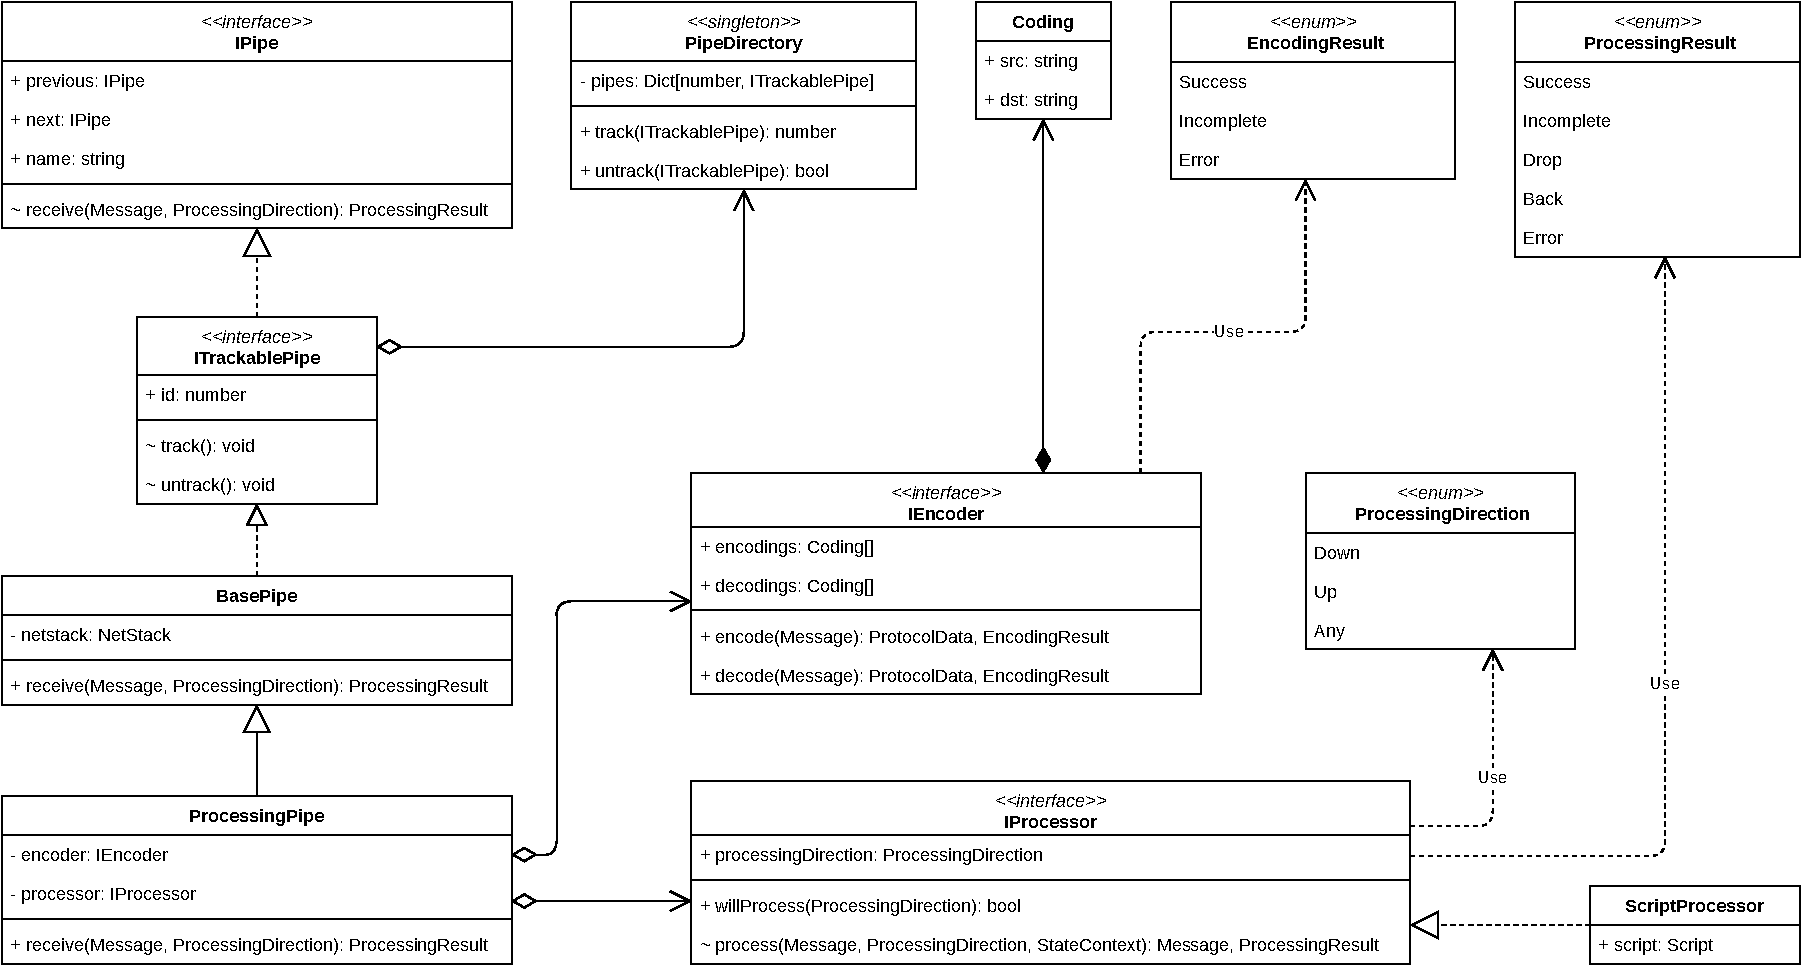
\includegraphics[height=12cm]{img/ch05/classes-2-pipes.pdf}
    \captionof{figure}{The interfaces, classes and enums used to represent pipes, their specializations and associated classes. This iteration separates BasePipes from IEncoders and IProcessors so BasePipes only implement routing of messages.}
    \label{fig:app-classes-2-pipes}
\end{sidewaysfigure}

\chapter{Interview Guideline}
\label{txt:app-interview-guideline}

\begin{enumerate}
    \item Experiences with IoT
          \begin{enumerate}\item Which technologies (software/protocols/platforms) were used in those applications?
              \item What context (home/industrial) were they used in?
              \item Were there any special constrains (e.g. real-time systems) when working with them?
              \item  How were the tests set up? (e.g. dedicated lab vs. on-site testing, single/multiple devices)
              \item Were those applications typical representatives for their field of use?
          \end{enumerate}
    \item   Processes in Everyday Life
          \begin{enumerate}\item  What are the goals and scopes of your penetration tests?
              \item  Which tasks do these goals typically involve?
              \item  Which tools do you use in the process and how regularly do you create specific tools yourself?
              \item  What problems do you typically face during tests?
              \item  Could specialized tools further improve your  everyday work? If so, what would those tools do?
          \end{enumerate}
    \item   The Future of IoT
          \begin{enumerate}\item  What do you think will IoT applications be like in the future? (e.g. regarding device specifications, cloud services, mobile integrations)
              \item What are the current challenges when working with IoT applications?
              \item  Lastly, what do you think will be future challenges when working with IoT?
          \end{enumerate}
\end{enumerate}